\section{Échantillonnage} % (fold)
\label{sec:échantillonnage}

	\paragraph{Drosophiles} % (fold)
	\label{par:drosophiles_mm}
	Nous échantillonons des souches de \esp{Wolbachia} ayant comme point commun d'être toutes très semblables à la souche \textit{wRi} infectant \esp{Drosophila simulans}, d'un point de vue nucléotidique. Elles seront souvent qualifiées de \emph{wRi-like}.

	\begin{figure}[h]
		\begin{center}
		\begin{tabular}{|c|c|c|}
			\hline
			\textbf{Hôte (souche)}			&\textbf{Déjà testées}				&\textbf{Nouvelles}\\
			\hline
			\esp{D. simulans} (wRi)	&Japon (Tokyo)				&Botswana\\
									&France (Grand Ferrade)		&Afrique du Sud\\
									&Portugal (Chicharo)		& \\
									&Mozambique (Chimoio)		& \\
			\hline
			\esp{D. melanogaster} (wMel)& USA (Seattle) 		& Botswanna (4 sites)\\
									&Pérou						&Zimbabwe\\
									&Madagascar					& \\
			\hline
			\esp{D. auraria} (wAur)	& Terrain (1 échantillon)	&Japon\\
			\hline
			\esp{D. triauraria} (wTriaur)&							&Japon\\
			\hline
			\esp{D. suzukii} (wSuz)	&							&France(6 sites)\\
									& 							&Japon\\
			\hline
			\esp{D. sub} (wSub)		&							&?\\
			\hline
		\end{tabular}
		\end{center}
		\caption{Tableau récapitulatif de la répartition spatiale des échantillons de drosophiles, ainsi que du nom de leurs \esp{Wolbachia} associées. En tout, 54 échantillons ont été typés en transposon-display}
		\label{fig:tab1}
	\end{figure}

	Les échantillons proviennent donc de plusieurs espèces de drosophiles, et de plusieurs points du globe (voir tableau \ref{fig:tab1}), en vue de situer les transferts horizontaux tant dans la dimention spatiale que phylogénétique.
	% paragraph drosophiles (end)

	\paragraph{\textit{L. heterotoma}} % (fold)
	\label{par:hetero_mm}
	\textit{L. heterotoma} étant dans la nature infectées par trois souches distinctes de \esp{Wolbachia}, il faut, pour typer celles-ci en Transposon-display, obtenir des lignées mono-infectées. Pour cela, nous appliquons une méthode basée sur des traitements antibiotiques ménagés, que nous décrivons en annexe, non décrits dans ce rapport.
	% paragraph hetero_mm (end)

% subsection échantillonnage (end)

\section{Extractions d'ADN et statuts d'infection} % (fold)
	Deux protocoles d'extractions d'ADN ont été suivies : 
	Pour la vérification des statuts d'infection, les extractions ont été faites en suivant le protocole Chelex®, méthode peu coûteuse mais produisant un matériel non purifié.

	L'efficacité de l'extraction a été vérifiée par le biais d'une PCR sur le gène \gene{Its2}, gène mitochondrien généraliste.

	Pour les besoins en précision du protocole du transposon-display, des extractions d'ADN produisant de l'ADN purifié ont dû être pratiqués, en suivant le protocole du kit \textit{NucleSpin® Tissue} de l’entreprise Macherey-Nagel.

	Les statuts d'infection ont été déterminés par PCR sur la base du gène \gene{FtsZ}\footnote{Amorces : FtsZ-F2/FtsZ-R2}.

	Pour certains échantillons de drosophiles, l'espèce exacte n'était pas déterminée de façon certaine sur la base de la morphologie. Elle a donc été déterminée sur la base du séquençage du produit de la PCR du gène mitochondrial \gene{COI}\footnote{Amorces~: LCO/HCO}, à partir des échantillons extraits au Chelex®.

	Puis, la caractérisation de la souche de la bactérie a été effectuée sur la base du gène \gene{wsp}\footnote{Amorces : 81F/2R}, connu pour sa variabilité au sein du genre \esp{Wolbachia}, fort utile pour le typage de la souche.

	Enfin, la présence du transposon \textit{ISWpi1} a été testée par PCR avec les amorces ISWpi1-F/ISWpi1-R.

\section{Transposon-display} % (fold)
\label{sec:transposon_display}

	\paragraph{Principe général} % (fold)
	\label{par:principe_TnDisp}
	Le transposon-display est une méthode de biologie moléculaire visant à établir un \textit{fingerprint} des locus d’insertion d’un transposon. 
	Elle est tirée de la méthode ASAP (Allele-Specific Alu PCR)\cite{ASAP}.
	Nous allons décrire ici brièvement son principe (voir le schéma \ref{fig:figure1})~:
	\begin{enumerate}
		\item Le génome est digéré par une enzyme de restriction (ici, HindIII), séléctionné pour couper fréquemment, mais pas dans le transposon.
		\item Des adaptateurs\footnote{Dessinés par Hélène \textsc{Henri}, décrits dans son mémoire \cite{memHH}} sont ensuite appliqués à cet ADN digéré, conçus pour être d’un côté complémentaires au motif de coupure de HindIII, et de l’autre pour ne pas être complémentaire sur la fin, afin de former un "Y" et d’éviter ainsi la circularisation.
		\item Nous nous retrouvons donc avec une série de fragments linéaires d’ADN de l’échantillon, flanqués de notre adaptateur, contenant pour certains le transposon qui nous intéresse (\textit{ISWpi2}).
		\item L’étape finale consiste en deux PCR, avec comme amorce commune une amorce spécifique à l’adaptateur (La partie en "Y"), et l’autre soit à la partie 5’ du transposon (ISb), soit la partie 3’ (ISc).
	\end{enumerate}
	% Le résultat (renvoyer à figure gels) de cette PCR, après éléctrophorèse, nous donne un \textit{barcode} dans lequel chaque bande correspond à un locus d’insertion du transposon.
	Après migration sur gel d’éléctrophorèse, nous obtenons un profil dans lequel chaque fragment correspond à un locus d’insertion du transposon.
	% paragraph principe_TnDisp (end)

	\paragraph{Des nouveautés dans le protocole} % (fold)
	\label{par:protocole2}
	Ce stage a été l’occasion pour tester une nouvelle version du protocole du transposon-display, en particulier au niveau de la PCR, avec l’utilisation d’une Taq-polymérase haute fidélité (AccuTaq de la société Sigma), et l’ajustement en conséquence du programme de thermocycleur.
	% paragraph protocole2 (end)

\begin{figure}[h!]
	\begin{center}
		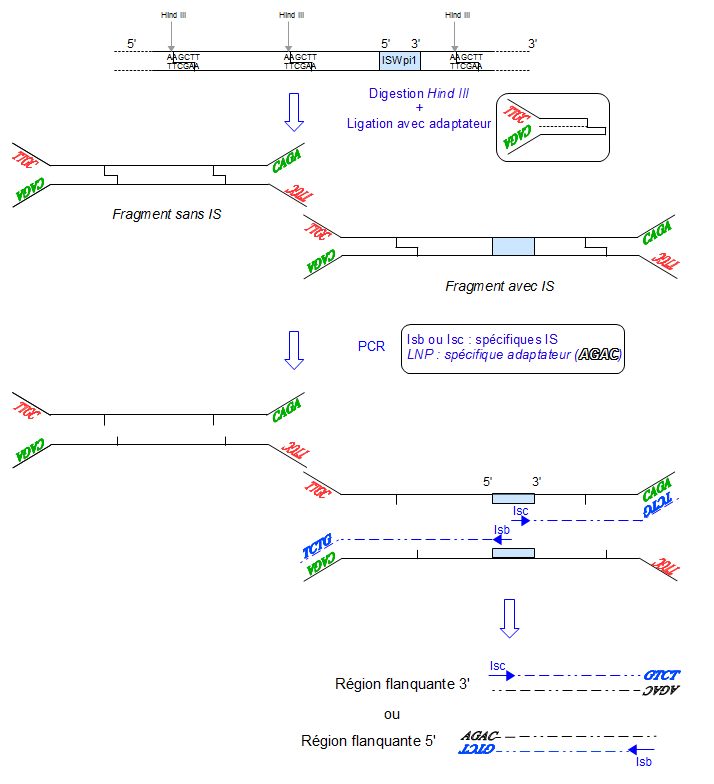
\includegraphics[width=160mm]{tdisplay.png}
	\end{center}
	\caption{Principe du Transposon Display avec amplification sélective des régions
flanquantes des insertions. Figure povenant du mémoire de Hélène \textsc{Henri}\cite{memHH}.% Là j'aimerais bien footciter, mais y'a un bug connu quand on footnote des trucs depuis une caption :(
	}
	\label{fig:figure1}
\end{figure}

% subsection transposon_display (end)
